\documentclass[12pt]{report}
\usepackage{blindtext}
\usepackage{hyperref}
\usepackage{tocloft}
\usepackage{natbib}
\usepackage{graphicx}
\usepackage[newfloat]{minted}
\usepackage{caption}
\usepackage{booktabs}
\usepackage[toc, page]{appendix}
\usepackage{multirow}
\usepackage{subcaption}
\newenvironment{longlisting}{\captionsetup{type=listing}}{}
\title{%
  GPT-2 Based Story Teller\\
  \large CTEC3451 Development Project \\~\\
    De Montfort University} 
\author{Artem Bobrov (P2547788)}
\date{May 5 2022}
\setlength{\parindent}{1em}
\begin{document}
\maketitle
\thispagestyle{empty}
\clearpage
\tableofcontents
\setcounter{tocdepth}{1}
\thispagestyle{empty}
\clearpage
\section*{Abstract}
\addcontentsline{toc}{section}{Abstract}
\paragraph{}
The project described in this report is a story-telling application that uses the GPT-2 model to generate text. 
The model is trained on multiple datasets and is able to generate text from a variety of topics in the backend. 
The frontend is a web application that allows users to endlessly generate stories accompanied by thematic pictures.
The point of the project is to prove the concept that neural networks, if trained properly, are able to generate 
data that is very similar to human language.

\section*{Introduction}
\addcontentsline{toc}{section}{Introduction}
\paragraph{}
Neural networks weren't so popular in the early days of computing, but they are now a common tool for machine learning.
First neural network was invented by Frank Rosenblatt in the late 1950s \citep{rosenblatt_1958_the}. Perceptron has only 
one layer of neurons, but more advance neural networks can have multiple layers. Before Transformer neural networks 
there were many different types of neural networks (e.g. Convolutional, Recurrent, LSTM, Feed Forward, etc).

Transformers were introduced in 2017 by Google \citep{attention_is_all_you_need} and are a new type of neural network. It uses self-attention mechanism 
to focus on the most relevant information in the input. It weights the significance of each part of the input differently.

This report focuses on the GPT-2 model, which is a transformer type neural network developed by OpenAI in 2019 \citep{radford_wu_child_luan_amodei_sutskever_2019}.
Despite the fact that GPT-3 is a newer model, it's predecessor is still a popular choice for text generation.

An application will be developed that utilises the features of GPT-2 and wraps it up in a user-friendly web
interface that allows users to read freshly generated stories accompanied by thematic pictures. The development process 
will be examined and the results will be presented and discussed in depth. The usage of the key elements and techniques used both in
backend and frontend will be explained. Moreover the project development and research cycle will be reflected on and 
other approaches that possibly could have been used to achieve different or similar results will be presented.

\clearpage

\section*{Objectives and Goals}
\addcontentsline{toc}{section}{Objectives and Goals}

\subsection*{Initial approach}
\addcontentsline{toc}{subsection}{Initial approach}
\paragraph{}
It is important to state that the original plan for the project was to develop a similar application that generates
pictures with attached text to them (known as `memes') and allows users to watch them using a web interface. It has been
planned to use different approach to build a repository of training data using `Optical Character Recognition (OCR)' \citep{tesseract_article} and 
`Pillow' library to attach processed text to the pictures. It has been decided to adjust the original plan and change the
topic from memes to stories.

\subsection*{New approach}
\addcontentsline{toc}{subsection}{New approach}
\paragraph{}
The new approach doesn't require any massive changes to the original plan and the project will be developed using the same
techniques - indetical frontend and almost the same backend. The only difference is that OCR will be removed from the backend
because it's not needed for the project anymore. To minimize the deviation from the original plan, there will be an
additional section in the web interface that creates `memes' based on novels and other piece of art.


\subsection*{Reasons}
\addcontentsline{toc}{subsection}{Reasons}
\paragraph{}
Despite the fact that many of the features used in the initial approach have been already developed - Tesseract OCR, 
Pillow Image placing, `Meme' scraper - one major issue made it extremely perplexing to continue the project without changing the approach.

The first puzzling part was hidden in reading the text (using Tesseract OCR) from the scraped images and translate them to text strings.
Memes contain text captions that makes it easy for a human to read, but this same process is hard for machines to do so - 
especially via OCR. There were some images successfully processed by it but it didn't satisfy the requirement because the the success rate was too low.
Many solutions were tried, but even pre-processing the images before feeding them to the OCR engine didn't seem to give much improvement.
The second complexity was to build a meme repository itself. Using the meme scraper is not the best solution because
the content obtained by it can be anything. Unfiltered, uncensored - it's a huge ethical problem.

\subsection*{General Description}
\addcontentsline{toc}{subsection}{General Description}
\paragraph{}
Two general components of the development project are described in two sections. Such apparent separation between these categories 
is due to the fact that this approach allows a simpler, faster and more effiecient implementation with better user
experience, it also improves code readability and maintainability.

The first one is the backend, which is responsible for generating text based on given datasets 
(stories, novels, other pieces of art, etc). It is implemented in Python and uses numerous libraries
to achieve the goal. Multiple steps are involved in generating simple text samples including hours of training.

The second component is the frontend, which is a web application that creates a user-friendly, simple interface
to scroll and read stories. It is implemented in JavaScript using many libraries, as well as the Python part.
Such approach to frontend was chosen because web development is flexible and it's easy to adapt to different
platforms. Also it's possible to extend it to a web service that doesn't require downloading the application
to user's computer.

The goal is create a system with pre-trained model, which the user can use to scroll through the stories and 
react to each story leaving a positive or a negative feedback - using the `Like' and `Dislike' buttons. Afterwards,
these reactions will be stored in a database to be used by the developer to understand which stories should be
corrected and improved. The feedback system is designed to create a reflection on the pre-trained model as a whole and
not on separate elements (stories). Given the feedback, the developer can decide to improve the model or not.

\clearpage

\section*{Major Components}
\addcontentsline{toc}{section}{Major Components}

\subsection*{Backend}
\addcontentsline{toc}{subsection}{Backend}
\paragraph{}
% General info - Python, PyCharm
The backend of the project is developed using Python programming language since it's a very popular language for machine learning
and has a lot of libraries that can be used to achieve the goal. The backend is developed using PyCharm IDE, which is also
a popular editor for Python. Calculations that are done in the backend can be executed on any machine with Python 
installed. The only issue is the optimisation - text generation requires a lot of computing power.

\subsubsection*{GPT-2 and the library}
\addcontentsline{toc}{subsubsection}{GPT-2 and the library}
\paragraph{}
% Libraries used to operate with the model
GPT-2 is the version of the GPT family used in the project. To operate with the network it was chosen to use a 
library called `GPT-2-simple' \citep{gpt-2-simple-git} since it features an easy approach to control and train the model.
The library is written in Python and offers a documentation which was used in order to work with the neural network.
GPT-2-simple offers two types of models - one with 124 million parameters and one with 324 million parameters. 
Acknowledging the computational limits of the processing unit used - graphical (GPU), the first model with 124 million
parameters was used. It is possible to use the second model but it requires a GPU with significantly more processing power and
memory. 

It is possible to use techniques that allow to save memory and train bigger models using memory saving gradients -
the main memory loss in the computation is due to calculating the gradient of the loss by backpropagation. At the
cost of one additional forward pass, the memory consumption can be reduced significantly \citep{chen_2016_training}.
However Tensorflow framework (version 2), which is used by GPT-2-simple, is not optimized for such tasks.

Despite providing simpler control functions, this library also provides a lot of tweaking options. For example, 
some of the hyperparameters can be changed to improve the model performance during testing. Learning rate, batch size,
number of training steps, number of accumulated gradients and optimizer can be changed. Number of layers and other
more complex parameters can also be changed but in order to do that, the parameters must be examined and adjusted in Tensorflow
code files.

The library also provides a way to load the model from a checkpoint file. This is useful when the model is trained
in multiple steps and it's needed to continue training from the last checkpoint without losing progress.

Another important feature for testing and optimising the output is the possibility to use different optimisers.
`Adam' and `SGD' are available optimisers. The first one is the most popular and is used in the project because 
the learning time is relatively short and the memory requirements are little \citep{musstafa_2022_optimizers}. 
These two aspects are crucial and thereforce the choice fell on `Adam'.

% Checkpoints, hyperparameters, adam


\subsubsection*{Datasets}
\addcontentsline{toc}{subsubsection}{Datasets}
\paragraph{}
% Alice, Catcher, Iliad, main problem - too much text decoration
Several datasets are used in the project. It has been chosen to use three datasets to work with. The first one is
the novel `Alice in Wonderland' by Lewis Carroll \citep{alice_in_wonderland}. This version was taken from GitHub Gist.
It's more adapted for machine learning than the original version since it's shorter and therefore contains less tokens.
For the reason that it was the first dataset to train the network on, it has been decided to go with the shortened version.
The text file with the novel poses a certain inconvenience because it contains a lot of text decoration which can create
noise in the model. But also it can have a positive effect on the user experience because it can be perceived as a
unique style of the author. The unformatted version contains 26,413 words and 148,574 characters.

The second dataset used is the novel `Catcher in the Rye' by J. D. Salinger \citep{catcher_in_the_rye}. The version found on GitHub is
slightly incomplete in the beginning and therefore was filled with the original text from the book. Also it was slightly
formatted for the sake of the correctness of the output of the neural network. Chapter enumeration and the title page
were removed from the text file. In the final revision there are 73,676 words and 382,008 characters.

The last and the longest dataset is the novel `Iliad' by Homer \citep{the_iliad}. It contains 152,507 words and 807,481 characters.
It doesn't contain much text decoration apart from chapter (book) enumeration. Also it has some translation references and copyright information.
All this information was removed from the dataset since it could affect the training process. It still can be viewed in the original text document 
in the reference list.

Later as the project evolves more datasets potentially could be added. The main problem of having multiple datasets is the size of the
checkpoint files created by the neural network for training purposes. `Alice in Wonderland' checkpoint, which was trained 3,200 times on the novel
is around 500MB and `Catcher in the Rye' checkpoint is about the same size and the same amount of training steps. It would be possible to add more stories to the
project if the checkpoint storage would be located not on the user's machine but rather on a server.

\subsubsection*{Pillow}
\addcontentsline{toc}{subsubsection}{Pillow}
\paragraph{}
% Meme section
`Pillow' is a Python library used to manipulate images \citep{pillow_lib}. It's a fork from an original library named
`PIL'. The reason why it was chosen to use in the development project is that it offers an easy and fast way
to insert text into the image. This process is also known as `meme' creation. It is possible to use generated samples
from the neural network, either cut the size of the samples after it has been generated or generate a small sample 
in the first place. The second option reduces the time of generation process but it also takes away the option
to format the text if the first and the last sentences are inappropriate. The customisation of the text in the library
is a very straightforward process. It is possible to change the font, the size, the colour, the position and the angle.
The `Meme mode' section will most likely contain pictures in unified format (i.e. the font size, the colour and the angle will
be the same).

In terms of the project, `Pillow' will be used in the `Meme mode' section. The idea is similar to the stories generator,
the difference lies in the fact that the text is inserted into the image, rather than being printed below the image.
Stories are presented in a post-like format.


\subsection*{Frontend}
\addcontentsline{toc}{subsection}{Frontend}
\paragraph{}
% HTML, CSS, JavaScript
The frontend of the project consists of a mixture of HTML, CSS and JavaScript. HTML is a markup language which is used
to create the layout of the webpage. CSS is a language used to style the webpage. In this project it's used in a
bundle with Bootstrap for easier manipulations with the styles. JavaScript is used to control the behaviour of
the webpage and everything in it. Some of the functions displayed in the webpage are calculated and controlled 
solely with JavaScript with no interaction with Python.

\subsubsection*{Web Application appearence}
\addcontentsline{toc}{subsubsection}{Web Application appearence}
\paragraph{}
% Bootstrap, Electron, theme change
The application appearance is based on Bootstrap 5 and Electron. Bootstrap \citep{bootstrap} is a CSS framework/library 
that is used to create a responsive and mobile-first design. It's files (CSS and JS) can be accessed via `Content 
Delivery Links' (CDN). This method is useful when only a part of the content hosted on CDN servers is used in
development since CDN technology allows to deliver only necessary files. Also a big advantage is the loading time
if the resource is server-based by reducing latency \citep{cdnetworks}. The other aspect of the look is `Electron' which
was formerly known as `Atom Shell' \citep{a2015_atom}. It's a cross-platform application that is used to develop
application with web-like design. The main reason to work with `Electron' is the ability to have the same look and feel
on all platforms. GUI applications can be developed and deployed using web technologies much faster. Prior to the introduction 
of `Electron' to the project, the application was developed on the basis of different browsers and operating systems.

Also as can be seen on the figures below, most popular approach to the development of Python GUI apps - Tkinter, doesn't
satisfy the standards of app design in early 2020s. 

\begin{figure}[ht]
  \captionsetup[subfigure]{labelformat=empty}
  \centering
  \begin{subfigure}{.5\textwidth}
    \centering
    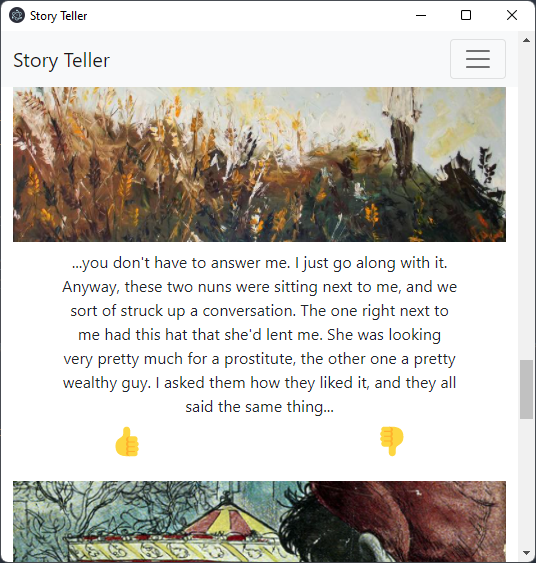
\includegraphics[width=.8\linewidth]{img/electron_window_example.png}
    \caption{Story Teller (Electron)}
    \label{fig:electron}
  \end{subfigure}%
  \begin{subfigure}{.5\textwidth}
    \centering
    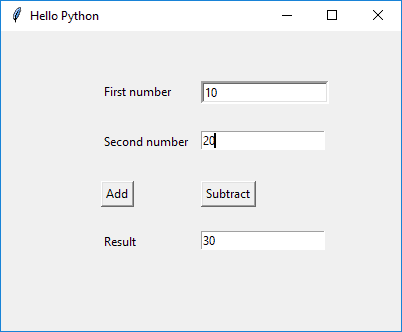
\includegraphics[width=.8\linewidth]{img/tkinter_window_example.png}
    \caption{Tkinter app}
    \label{fig:tkinter}
  \end{subfigure}
  \caption{A comparison of two GUI layouts}
  \label{fig:comparison_tk_electron}
\end{figure}

\clearpage

Similar situation occurs when it comes to animation with Tkinter. Many examples and many guides were examined and 
it has been concluded that Tkinter, in spite of the fact that it's one of the most popular GUI libraries, is not
suitable for the purpose of the project because the aim of the project is to create a fancy web-based application
that can catch the attention of the user.

Another aspect of the design is the theme. Since many modern projects offer a possibility to change to 
either a light or a dark theme, it has been decided to develop an application with two themes. Bootstrap 
does most of the work for the theme change in terms of the colour change. Theme is persistent and is to a
settings file which is stored in the application's folder. On every start-up the application checks if the
theme is set to the light or dark mode accessing the JSON file.

\begin{figure}[ht]
  \captionsetup[subfigure]{labelformat=empty}
  \centering
  \begin{subfigure}{.5\textwidth}
    \centering
    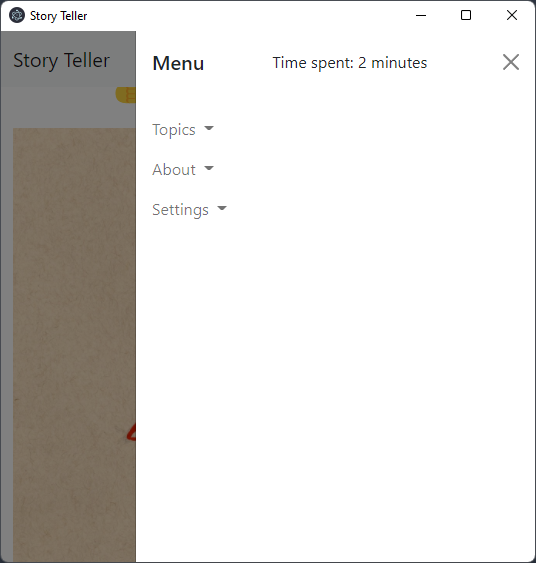
\includegraphics[width=.8\linewidth]{img/light_theme.png}
    \caption{Light theme}
    \label{fig:light_theme}
  \end{subfigure}%
  \begin{subfigure}{.5\textwidth}
    \centering
    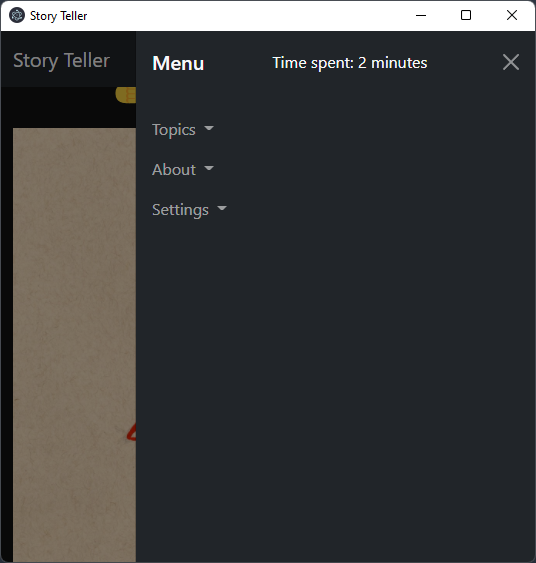
\includegraphics[width=.8\linewidth]{img/dark_theme.png}
    \caption{Dark theme}
    \label{fig:dark_theme}
  \end{subfigure}
  \caption{A comparison of two GUI themes}
  \label{fig:comparison_light_dark}
\end{figure}



\subsubsection*{Displaying the content}
\addcontentsline{toc}{subsubsection}{Displaying the content}
\paragraph{}
% Lazy loading, formatting the NN output, JQuery
To display the content it has been chosen to follow modern techniques of infinite scrolling. It loads
the content continously while the content is being generated on the fly. Infinite scrolling absolutely matches the 
topic of the project since the main idea was to create stories without any administrator intervention and 
minimise any unnecessary clicks and interactions. The content is displayed in a post-like format - that means 
a random picture from a set is followed by a random and freshly generated text based on a neural network checkpoint.
The displayed content depends on which topic is selected since the content is separated in different topics and 
displayed with different pictures.

Another aspect which was considered with exclusive scrupulousness is the conformity to accepted social standards. 
In view of the fact that neural networks do not understand major human problems of inequality, supremacism and just 
unacceptable language, a word filter can be used to filter out the most offensive words. A dictionary of such words
can be formed and used to exclude the possible offensive language. Some content fed to the network might contain
questionable statements and thus the output of the network will contain altered but still questionable words.
The problem might be regarded from two perspectives: the first one is that it's not acceptable and the second one
is that it's not even a problem because the output is generated based on the style of the original author. 


\subsubsection*{User feedback}
\addcontentsline{toc}{subsubsection}{User feedback}
\paragraph{}
% Like and dislike buttons
User feedback is an easy and effective way to improve the application and enhance the text generation process in
particular. To establish a dialogue with a user the application uses a standard approach to the problem.
The user can either like or dislike the text generated by the application by simply clicking one of the buttons. 
It is planned to store the reactions in the database and use them to manually assess the quality of the content.
Comments are another possible solution to the user feedback problem but they seem too like a too complicated
approach.

\subsubsection*{Database}
\addcontentsline{toc}{subsubsection}{Database}
\paragraph{}
% Storing settings, user feedback, theme change, JSON
Databases are used to store the user settings and the user feedback. The settings are stored in a JSON file and are
accessed every time the application is started. JSON is a lightweight, human-readable text format that can be used with
any programming language. The objects in the files are stored in an `attribute-value' format. 

The purpose of the traditional database is defeated since the application doesn't store any sensitive information.
No encryption of the database is used either.

\clearpage

There are many other data serialisation formats such as XML, YAML, BSON etc. It has been decided to use JSON because
of its simplicity and flexibility compared to YAML. YAML is a superset of JSON and it seemed to big for the purpose.

\begin{figure}[ht]
  \centering
  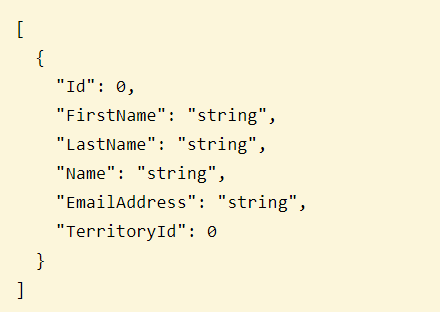
\includegraphics[width=0.5\linewidth]{img/json_example.png}
  \caption{JSON database}
  \label{fig:json}
\end{figure}

\subsection*{Linking the frontend and backend}
\addcontentsline{toc}{subsection}{Linking the frontend and backend}
\paragraph{}
% Eel, Python, JavaScript
The main bridge between the frontend and backend used in this project is a `little Python library' 
called `Eel' \citep{knott_2022_eel}. It allows interaction between JavaScript and Python at every point of
the development. The library is used to create a web server that can be accessed from the browser - 
Chrome, Safari, Firefox and last but not least - Electron. 

The most important feature of `Eel' is function exposition. It allows to call any function that is explicitly 
defined with a `@eel.expose' decorator and use it anywhere in the JavaScript code and vice versa.

\begin{figure}[ht]
  \centering
  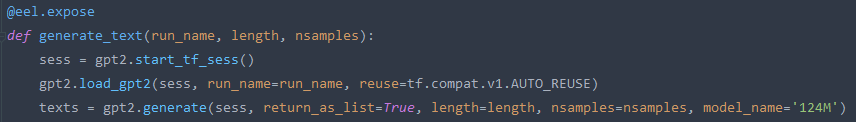
\includegraphics[width=1\linewidth]{img/eel_expose_example.png}
  \caption{Eel exposition}
  \label{fig:eel}
\end{figure}

It's important to note that when a function call is made from the JavaScript code, it should be done in
async/await fashion. This is because the function call is made in the background and the result is returned
after some time.

The separation of the frontend and backend is an important action becasue it allowed to use the most efficient
approaches on each side and also focus on each part individually.

\begin{figure}[ht]
  \centering
  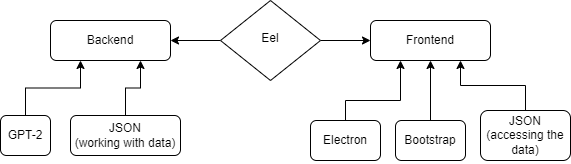
\includegraphics[width=1\linewidth]{img/system_diagram.png}
  \caption{The relations in the system}
  \label{fig:system_diagram}
\end{figure}

\clearpage

\section*{Development lifecycle}
\addcontentsline{toc}{section}{Development lifecycle}
\paragraph{}
Development process followed the principles of Agile practice. The main aspects of the development methodology
are: continiual improvement, flexible responses to any change and most importantly evolutionary development. Since
the project is developed by a single person, not a team, some of the practices of agile methodology are not applicable.


% \subsection*{Building the input repository}
% \addcontentsline{toc}{subsection}{Building the input repository}
% \paragraph{}


% Training sprint
% Implementation
% Testing
\subsection*{Training the model}
\addcontentsline{toc}{subsection}{Training the model}
\subsubsection*{Implementation}
\addcontentsline{toc}{subsubsection}{Implementation}
\paragraph{}
Training or finetuning the model was a crucial step in the development process. Before the neural network would
be able to generate specific text based on some dataset, it has to be trained on it. The training process involves
tweaking many parameters of the model and the process is repeated until the best options are found. Currently,
all three checkpoints are trained with the same parameters and on the same model - 124M (124 million parameters). 
The finetuning process begins with a creation of a new session. Then the the finetuning function itself is called
with the following parameters: \textit{dataset name, model name, number of steps, name of the run, restore point,
overwrite option, length of the sample and an interval to save the checkpoints}.

Dataset name is the name of the preferred text file to train the network on. For this project three datasets were
chosen - Alice, Catcher and Iliad. Model name is the name of the model used in the training process. It can be either
`124M' or `355M'. The difference is in the parameter count. The `124M' model has 124 million parameters while the
`355M' model has 355 million parameters. Number of steps is the parameter that determines how many times will the
training process be repeated. For this project every checkpoint is trained more than 3,000 times in order to
produce a meaningful result. Run name parameter specifies which checkpoint is being trained. It is useful to have
multiple runs in the same model. Restore point and overwrite options are used for the sake of optimisation of the
process to minimise the chance of failing (crashing). Also the interval to save the checkpoints is set to a small
value of 100 to save the progress in case the process crashes.

\begin{figure}[ht]
  \centering
  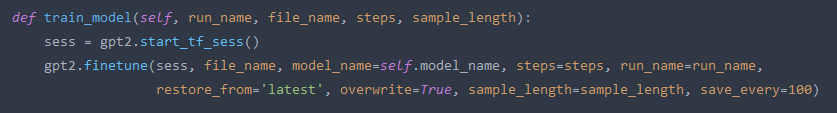
\includegraphics[width=1\linewidth]{img/train_model_example.png}
  \caption{Training function}
  \label{fig:train_model}
\end{figure}

\clearpage

\subsubsection*{Testing}
\addcontentsline{toc}{subsubsection}{Testing}
\paragraph{}

Testing \hyperref[appendix:model_testing]{appendix}


% IMPLEMENTATION:
% Building repository
% Training the model
% Generating text (best samples)
% Testing
% Code explanation
% Examples

%TC:ignore

\addcontentsline{toc}{section}{Bibliography}
\bibliography{reference}{}
\bibliographystyle{agsm}

\begin{appendices}
\section*{Testing}
\addcontentsline{toc}{section}{Testing}
\subsection*{Model testing}
\addcontentsline{toc}{subsection}{Model testing}
\label{appendix:model_testing}

\begin{table}[ht]
  \centering
  \begin{tabular}{@{\extracolsep{1pt}}lllll}
  \toprule   
  {Case} & {Input} & {Expected} & {Actual} & {Result}\\
  \midrule
  \multirow{3}{*}{GEN0} & Length: 10 & \multirow{2}{*}{No cut text} & \multirow{2}{*}{Text cut} & \multirow{2}{*}{Fail}\\ 
  & Samples: 1 & \multirow{2}{*}{Time: $<$15s} & \multirow{2}{*}{Time: 6.64s} & \multirow{2}{*}{Pass}\\
  & Batches: 1 &  & & \\
  \addlinespace[3pt]
  \multirow{3}{*}{GEN1} & Length: 1023 & \multirow{2}{*}{No cut text} & \multirow{2}{*}{Text cut} & \multirow{2}{*}{Fail}\\ 
  & Samples: 1 & \multirow{2}{*}{Time: $<$15s} & \multirow{2}{*}{Time: 12.99s} & \multirow{2}{*}{Pass} \\
  & Batches: 1 & & & \\
  \addlinespace[3pt]
  \multirow{3}{*}{GEN2} & Length: 500 & \multirow{2}{*}{No cut text} & \multirow{2}{*}{Text cut} & \multirow{2}{*}{Fail}\\ 
  & Samples: 6 & \multirow{2}{*}{Time: $<$15s} & \multirow{2}{*}{Time: 30.48s} & \multirow{2}{*}{Fail} \\
  & Batches: 1 & & & \\
  \addlinespace[3pt]
  \multirow{3}{*}{GEN3} & Length: 64 & \multirow{2}{*}{No cut text} & \multirow{2}{*}{Text cut} & \multirow{2}{*}{Fail}\\ 
  & Samples: 2 & \multirow{2}{*}{Time: $<$15s} & \multirow{2}{*}{Time: 5.41s} & \multirow{2}{*}{Pass} \\
  & Batches: 2 & & & \\
  \addlinespace[3pt]
  \multirow{3}{*}{GEN4} & Length: 60 & \multirow{2}{*}{No cut text} & \multirow{2}{*}{Text cut} & \multirow{2}{*}{Fail}\\
  & Samples: 2 & \multirow{2}{*}{Time: $<$15s} & \multirow{2}{*}{Time: 5.33s} & \multirow{2}{*}{Pass} \\
  & Batches: 2 & & & \\
  \addlinespace[3pt]
  \multirow{4}{*}{GEN5} & Length: 60 & \multirow{2}{*}{No cut text} & \multirow{2}{*}{Text cut} & \multirow{2}{*}{Fail}\\
  & Samples: 2 & \multirow{2}{*}{Time: $<$15s} & \multirow{2}{*}{Time: 5.43s} & \multirow{2}{*}{Pass} \\
  & Batches: 1 & & & \\
  \addlinespace[3pt]
  \multirow{4}{*}{GEN6} & Length: 70 & \multirow{2}{*}{No cut text} & \multirow{2}{*}{Text cut} & \multirow{2}{*}{Fail}\\
  & Samples: 2 & \multirow{2}{*}{Time: $<$15s} & \multirow{2}{*}{Time: 5.63s} & \multirow{2}{*}{Pass} \\
  & Batches: 1 & & & \\
  \addlinespace[3pt]
  \multirow{4}{*}{GEN7} & Length: 100 & \multirow{2}{*}{No cut text} & \multirow{2}{*}{Text cut} & \multirow{2}{*}{Fail}\\
  & Samples: 6 & \multirow{2}{*}{Time: $<$15s} & \multirow{2}{*}{Time: 9.46s} & \multirow{2}{*}{Pass} \\
  & Batches: 1 & & & \\
  \bottomrule
  \end{tabular}
  \caption{`Alice' (3100 steps) dataset text generation testing} 
\end{table}




\clearpage

\section*{Appendix B}
\label{appendix:B}
\addcontentsline{toc}{section}{Appendix B}

\end{appendices}

%TC:endignore

\end{document}